\section{Geometrische simpliziale Komplexe und Triangulierung}
\begin{thDef}[Affin (un-)abhängig]
    Sind $n,d\in\N$ und $v_0,\ldots,v_n\in\R^d$, so bezeichnen wir diese
    Vektoren als \emph{affin abhängig}, falls es Elemente
    $\lambda_0,\ldots,\lambda_n \in\R$ mit folgenden drei Eigenschaften gibt:
    \[ \textstyle
        \{\lambda_0,\ldots,\lambda_n\} \neq \{0\}, \quad \isum^n \lambda_i = 0
        \qundq \isum^n \lambda_i\,v_i = 0 \in\R^d
    . \] 
    Falls es solche Zahlen nicht gibt, so bezeichnen wir die Vektoren als
    \emph{affin unabhängig}.
\end{thDef}

\begin{thDef}[Konvexe Menge, konvexe Hülle]
    Sei $d\in\N$. Eine Teilmenge $A\subset\R^d$ heißt \emph{konvex}, wenn
    für alle $x,y\in A$ auch die (lineare) Verbindungsstrecke
    $\{ tx + (1-t)\,y \Mid t\in[0,1] \}$ in~$A$ enthalten ist.
    Für eine Teilmenge $A'\subset\R^d$ definiert
    $ \conv(A') \defeq 
        \bigcap \,\bigl\{ A\subset\R^d \Mid A'\subset A\text{ konvex} \bigr\}
    $
    die \emph{konvexe Hülle von $A'$}.
\end{thDef}

\begin{thDef}[(Geometrisches) Simplex, Seite]
    \label{gsc:def:simplex}
    %
    \hfill
    \begin{itemize}
        \item
            Sei $d\in\N$. Ein Simplex~$\sigma$ ist die konvexe Hülle $\conv(A)$ einer 
            endlichen Teilmenge $A\subset\R^d$ affin unabhängiger Vektoren.
            Die Elemente aus $A$ nennen wir \emph{Eckpunkte (von~$\sigma$)}. 
            Die \emph{Dimension von~$\sigma$} ist dann durch 
            $\dim(\sigma) \defeq \abs{A}-1$ definiert.
        \item
            Eine \emph{Seite von $\sigma$} ist ein Simplex $\conv(A')$ mit
            $A'\subset A$.
    \end{itemize}
\end{thDef}
%
%\begin{center}
%    \begin{tikzpicture}[%
%            scale=0.5,
%            mypoint/.style={shape=circle, inner sep=1.1pt, color=black, fill}
%        ]
%        \begin{scope}
%            \node at (0,0) [mypoint] {};
%        \end{scope}
%        \begin{scope}[shift={(2.5,0)}]
%            \draw (0,0) node [mypoint] {} -- (1,0) node [mypoint] {};
%        \end{scope}
%        \begin{scope}[shift={(6,0)}]
%            \draw [fill=black!20] (0,0) node [mypoint] {} -- 
%                  (1,0) node [mypoint] {} --
%                  (0.5,1) node [mypoint] {} -- cycle ;
%        \end{scope}
%        \begin{scope}[shift={(9.7,0)},z={(-5mm,-4mm)}]
%            \coordinate (A) at (0,0,1);
%            \coordinate (B) at (1,0,0);
%            \coordinate (C) at (0,1,0);
%            \coordinate (D) at (0,0,0);
%            
%            \draw [fill=black!20]
%                  (A) node [mypoint] {} --
%                  (B) node [mypoint] {} --
%                  (C) node [mypoint] {} -- cycle
%                  (D) node [mypoint] {};
%            \draw [dash pattern=on \pgflinewidth off 0.6pt] (A) -- (D) -- (C) (D) -- (B);
%        \end{scope}
%    \end{tikzpicture}
%    \\
%    \footnotesize
%    $0$- bis $3$-dimensionale Simplizes
%\end{center}

\begin{thDef}%
    [Geometrischer simplizialer Komplex]
    \label{gsc:def:gsc}
    %
    Sei $d\in\N$. 
    Ein \emph{geometrischer simplizialer Komplex} ist eine nicht-leere
    Menge~$\Delta$ von Simplizes im $\R^d$, welche folgende Bedingungen erfüllt:
    \begin{itemize}
        \item Ist $\sigma$ ein Simplex in $\Delta$, so ist auch jede Seite von
            $\sigma$ in $\Delta$ enthalten.
        \item
            Der Schnitt zweier Simplizes $\sigma_1,\sigma_2\in\Delta$ ist eine
            Seite von $\sigma_1$ und $\sigma_2$.
    \end{itemize}
    Wir setzen
    $\polyeder\Delta \defeq \bigcup \Delta \;\subset\R^d$
    und statten diesen Raum mit folgender Topologie aus:
    $A\subset\polyeder\Delta$ ist genau dann offen (abgeschlossen), wenn für alle
    $\sigma\in\Delta$ der Schnitt $A\cap\sigma$ offen (abgeschlossen) in
    $\sigma$ ist (wobei $\sigma$ die Teilraumtopologie trägt). Wir nennen dann
    $\polyeder\Delta$ das \emph{zu $\Delta$ gehörige Polyeder}.
\end{thDef}

\begin{center}
    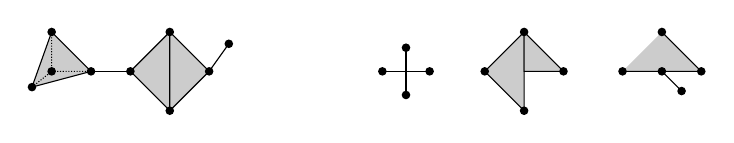
\begin{tikzpicture}[%
            scale=0.5,
            mypoint/.style={shape=circle, inner sep=1.1pt, color=black, fill}
        ]
        \begin{scope}[z={(-5mm,-4mm)}]
            \coordinate (A) at (0,0,1);
            \coordinate (B) at (1,0,0);
            \coordinate (C) at (0,1,0);
            \coordinate (D) at (0,0,0);
            
            \coordinate (E) at (2,0,0);
            \coordinate (F1) at (3,1,0);
            \coordinate (F2) at (3,-1,0);
            \coordinate (G) at (4,0,0);
            \coordinate (H) at (4.5,0.7,0);
            
            \draw [fill=black!20]
                  (A) node [mypoint] {} --
                  (B) node [mypoint] {} --
                  (C) node [mypoint] {} -- cycle
                  (D) node [mypoint] {};
            \draw [dash pattern=on \pgflinewidth off 0.6pt] (A) -- (D) -- (C) (D) -- (B);
            
            \draw (B) -- (E);
            \draw [fill=black!20] (E) -- (F1) -- (F2) -- cycle;
            \draw [fill=black!20] (G) -- (F1) -- (F2) -- cycle;
            \path (E)  node [mypoint] {} 
                  (F1) node [mypoint] {}
                  (F2) node [mypoint] {};
            
            \draw (G) node [mypoint] {} -- (H) node [mypoint] {};
        \end{scope}
        
        \begin{scope}[xshift=1cm]
        \begin{scope}[shift={(8,0)},scale=0.6]
            \draw (-1,0) node [mypoint] {} -- (1,0) node [mypoint] {}
                  (0,-1) node [mypoint] {} -- (0,1) node [mypoint] {};
        \end{scope}
        
        \begin{scope}[shift={(8,0)}]
            \coordinate (E) at (2,0);
            \coordinate (F1) at (3,1);
            \coordinate (F2) at (3,-1);
            \coordinate (F3) at (3,0);
            \coordinate (G) at (4,0);
            
            \draw [fill=black!20] (E) -- (F1) -- (F2) -- cycle;
            \draw [fill=black!20] (G) -- (F1) -- (F3) -- cycle;
            \path (E)  node [mypoint] {} 
                  (F1) node [mypoint] {}
                  (F2) node [mypoint] {}
                  (G)  node [mypoint] {};
        \end{scope}
        
        \begin{scope}[shift={(13.5,0)}]
            \draw [fill=black!20] 
                (0,0) node [mypoint] {} --
                (2,0) node [mypoint] {} -- 
                (1,1) node [mypoint] {};
            \draw (1,0) node [mypoint] {} -- (1.5,-0.5) node [mypoint] {};
        \end{scope}
        \end{scope}
    \end{tikzpicture}
    \\
    \footnotesize
    Simplizialer Komplex (links) und 
    \emph{keine} simplizialen Komplexe (rechts)
\end{center}

\begin{thAufgabe}
    Fügen Sie derart Simplizes zu den obigen Gegenbeispielen hinzu, so dass
    diese zu simplizialen Komplexen werden. Versuchen Sie nun dasselbe zu
    erreichen, indem Sie (möglichst wenige) Simplizes entfernen.
\end{thAufgabe}

\begin{thDef}[Triangulierbar, Triangulierung]
    Ein topologischer Raum~$X$ heißt \emph{triangulierbar}, falls es
    einen simplizialen Komplex $\Delta$ und einen Homöomorphismus
    $\polyeder\Delta \cong X$ gibt. Solch einen Homöomorphismus nennen wir 
    eine \emph{Triangulierung von $X$}.
\end{thDef}

\begin{thBeispiel}\label{gsc:bsp:spheretriang}
    Zu $d\in\N[\geq1]$ erhalten wir eine Triangulierung der Sphäre
    $S^{d-1}$ wie folgt: Sei $\sigma$ ein $d$-dimensionales Simplex. Wir bilden
    dann den zugehörigen simplizialen Komplex und entfernen die einzige
    $d$-dimensionale Seite (also $\sigma$ selbst). Wir erhalten so einen
    simplizialen Komplex $\Delta(\sigma)\setminus\{\sigma\}$, dessen Polyeder
    (vermöge einer Zentralprojektion) zur Einheitssphäre~$S^{d-1}$ homöomorph ist. 
\end{thBeispiel}

\enlargethispage{1.5cm}
\begin{center}
    \begin{tikzpicture}[scale=2]
        \draw (0,0) -- (1,0) -- ++(120:1) -- cycle;
        \path [name path=m1] (0,0) -- (30:1);
        \path [name path=m2] (1,0) -- ++(150:1);
        \path [name intersections={of=m1 and m2,by=C}];
        \draw let \p1=(C), \n1 = {veclen(\x1,\y1)} in (C) circle [radius=\n1];
        
        \foreach \ang in {0,30,...,330} 
            \draw let \p1=(C), \n1 = {veclen(\x1,\y1)} in
                [->, color=black!40, opacity=0.65, densely dotted]
                (C) -- +(\ang:\n1);
            
        \node [align=center] at (2,0.3) {\footnotesize Triangulierung\\
                                       \footnotesize der $1$-Sphäre};
    \end{tikzpicture}%
\end{center}
